\documentclass{article}
\usepackage{graphicx}
\usepackage[margin=1.5cm]{geometry}
\usepackage{amsmath}

\begin{document}

\title{Warm Up: Graphical Analysis of Kinematics}
\author{Prof. Jordan C. Hanson}

\maketitle

\begin{figure}
\centering
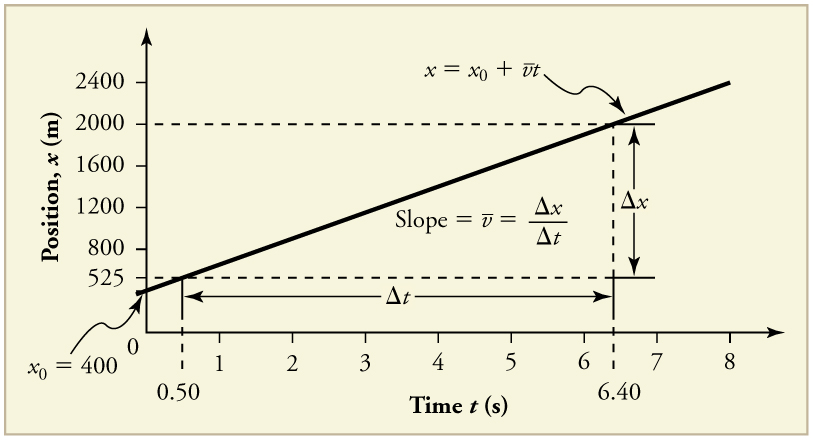
\includegraphics[width=0.45\textwidth]{figures/slope.jpeg} \hspace{1cm}
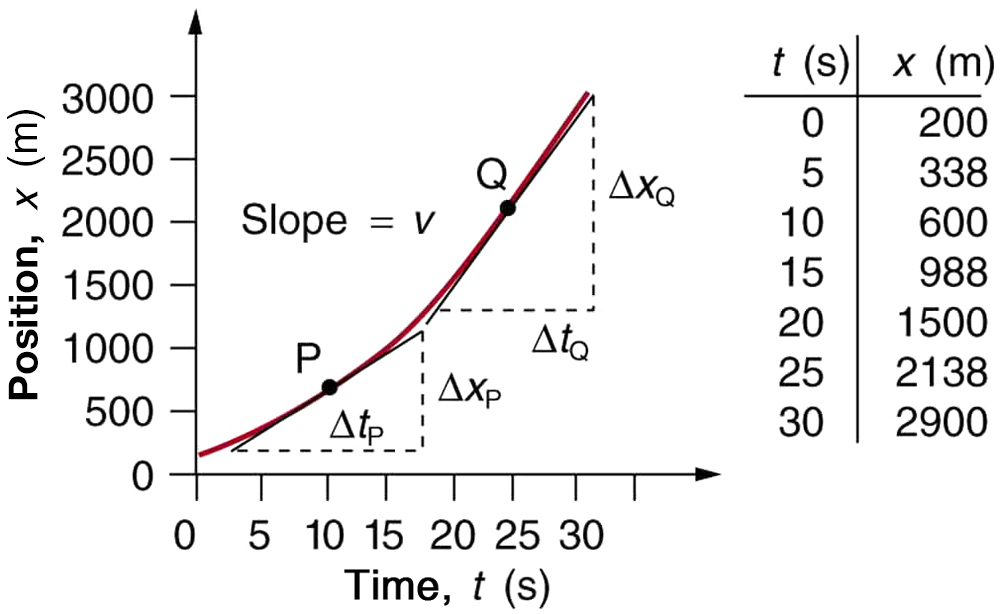
\includegraphics[width=0.45\textwidth]{figures/slope2.jpeg}
\caption{\label{fig:1} (Left) A system moves with constant velocity.  Velocity is the slope on this plot. (Right) A system moves with non-constant velocity.}
\end{figure}

\section{Memory Bank}

\begin{enumerate}
\item $v = \frac{\Delta x}{\Delta t}$ ... Average velocity.
\item $x(t) = v t + x_i$ ... Position versus time with constant velocity.
\item $a = \frac{\Delta v}{\Delta t}$ ... Acceleration is the change in velocity.
\end{enumerate}

\section{Chapter 2 - Graphical Analysis of Kinematics}

\begin{enumerate}
\item Consider the motion of the system depicted in Fig. \ref{fig:1} (Left).  What is the speed of the system?  Suppose the system is moving in the positive y-direction.  What is the expression of the velocity? \\ \vspace{1cm}
\item Write an equation for the position of the system in Fig. \ref{fig:1} (Left) versus time.  Where will the system be at 18 seconds? \\ \vspace{1cm}
\item Consider the motion of the system in Fig. \ref{fig:1} (Right).  Find the change in velocity between points P and Q.  Calculate the acceleration.  \textit{Hint: pay attention to units.}
\end{enumerate}

\end{document}
